\documentclass[12pt,spanish]{article}
\usepackage[spanish]{babel}
\usepackage{graphicx}
\usepackage{color}
\usepackage{xcolor}
\usepackage{colortbl}
\usepackage{amsthm,thmtools}
\usepackage{multirow}
\usepackage{amsmath}
\usepackage{subcaption}
\usepackage{adjustbox}
\usepackage{multirow}
\usepackage[hidelinks]{hyperref}
\usepackage{caption}
\usepackage{amsthm}
\usepackage{multicol}
\usepackage[outputdir=build]{minted}
\usepackage{float}
\usepackage{amsfonts}
\usepackage{enumitem}
\usepackage{titling}
\usepackage{soul}
\usepackage{listings}
\usepackage{array}
\graphicspath{ {./img/} {../../LaTeX/img/}}
\selectlanguage{spanish}
\usepackage[utf8]{inputenc}
\usepackage{graphicx}
\newmintedfile[cppcode]{c++}{
linenos=true,
breaklines=true,
tabsize=2,
}

\newmintedfile[script]{bash}{
linenos=true,
breaklines=true,
tabsize=2,
}

\usepackage[a4paper,left=2cm,right=2cm,top=2.5cm,bottom=2.5cm]{geometry}


\makeatletter
\patchcmd\thmt@mklistcmd
  {\thmt@thmname}
  {\check@optarg{\thmt@thmname}}
  {}{}
\patchcmd\thmt@mklistcmd
  {\thmt@thmname\ifx}
  {\check@optarg{\thmt@thmname }\ifx}
  {}{}
\protected\def\check@optarg#1{%
  \@ifnextchar\thmtformatoptarg\@secondoftwo{#1}%
}
\makeatother





\title{Inteligencia Artificial}
\setlength{\droptitle}{10em}
\author{Carlos Sánchez Páez}

\makeindex
\begin{document}


\begin{titlepage}

\newlength{\centeroffset}
\setlength{\centeroffset}{-0.5\oddsidemargin}
\addtolength{\centeroffset}{0.5\evensidemargin}
\thispagestyle{empty}

\noindent\hspace*{\centeroffset}
\begin{minipage}{\textwidth}

\centering

\includegraphics[width=0.9\textwidth]{logo_ugr.jpg}\\[1.4cm]

\textsc{ \Large Inteligencia Artificial\\[0.2cm]}
\textsc{GRADO EN INGENIERÍA INFORMÁTICA}\\[1cm]

{\Huge\bfseries Práctica 3.\\
}
\noindent\rule[-1ex]{\textwidth}{3pt}\\[3.5ex]
{\large\bfseries Jugador automático para Mancala}
\end{minipage}

\vspace{1.5cm}
\noindent\hspace*{\centeroffset}
\begin{minipage}{\textwidth}
\centering

\textbf{Autor}\\ {Carlos Sánchez Páez}\\[2.5ex]

\includegraphics[width=0.3\textwidth]{etsiit_logo.png}\\[0.1cm]
\vspace{1.5cm}

\includegraphics[width=0.5\textwidth]{decsai.jpg}\\[0.1cm]
\vspace{1cm}
\textsc{Escuela Técnica Superior de Ingenierías Informática y de Telecomunicación}\\
\vspace{1cm}
\textsc{Curso 2017-2018}
\end{minipage}
\end{titlepage}
\thispagestyle{empty}
\newpage
\tableofcontents{}
\newpage
\thispagestyle{empty}



\section{Introducción}

Esta práctica consiste en la implementación de un agente deliberativo que tendrá que actuar en un entorno multi-agente competitivo con el objetivo de ganar. Trabajaremos sobre el juego \emph{Mancala}.

\begin{figure}[H]
\centering
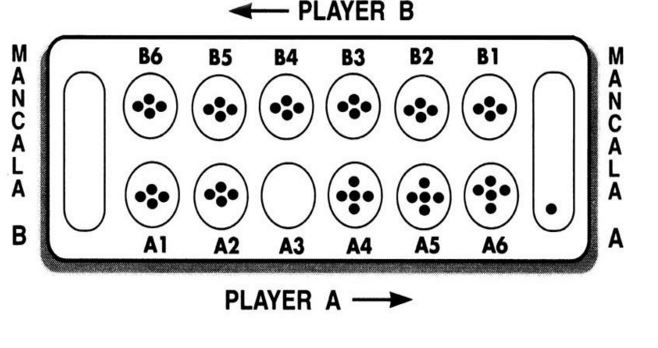
\includegraphics[scale=0.5]{mancala.png}
\caption{Tablero de Mancala.}
\end{figure}

\section{Estructuras, constantes y métodos auxiliares}

\begin{minted}[linenos,tabsize=2,breaklines]{c++}
struct node {
  GameState estado;	//Estado
  Move movimiento;	//Movimiento que lo ocasionó
};
const vector<Move> MOVIMIENTOS = {M1, M2, M3, M4, M5, M6};//Posibles movimientos.
const vector<Position> POSICIONES = {P1, P2, P3, P4, P5, P6};//Posiciones de cada jugador.
const int PROFUNDIDAD_MAXIMA = 8;//Profundidad límite. Llega a 135.145 nodos generados como máximo.
Player oponente, yo;	//Variables de control de la clase
bool primera_vez = true;	//Primera vez que se ejecuta nextMove().
const int MIN = numeric_limits<int>::min();	// -INF
const int MAX = numeric_limits<int>::max();//  +INF
//Métodos auxiliares
int Maximo(int a, int b) const;
int Minimo(int a, int b) const;
bool Podar(int alpha, int beta) const;	//True si se cumple el criterio de poda.
bool Inmolacion(const GameState &estado, const Move &mov) const; //True si intentamos inmolarnos (sembrar en una casilla en la que no hay semillas).
\end{minted}
\captionof{figure}{Estructuras, constantes y métodos auxiliares.}




\section{Algoritmo empleado}

El algoritmo empleado para resolver la práctica es el \textbf{minimax} con el añadido de la \textbf{poda $\alpha$-$\beta$} para conseguir mayor optimalidad.\\

Como se nos da un límite de tiempo para cada turno, estamos obligados a realizar un cálculo heurístico de la calidad de los distintos movimientos. 


\subsection{Algoritmo minimax con poda $\alpha$-$\beta$}

El algoritmo se apoya en dos métodos: uno principal que será llamado cuando sea el turno de nuestro bot (se encargará de expandir la raíz del árbol de estados) y otro recursivo que explorará los correspondientes hijos.\\

El funcionamiento del algoritmo principal es el siguiente:

\begin{enumerate}
	\item Genero los hijos del nodo raíz.
	\item Inicializo $\alpha=-\infty$ y $\beta=+\infty$.
	\item Para cada hijo:
		\begin{enumerate}[label=3.\arabic*]
			\item Compruebo si será mi turno. En caso afirmativo, será un nodo a maximizar.
			\item Calculo el valor heurístico del hijo mediante el algoritmo recursivo.
			\item Si obtengo un valor mayor que $\alpha$, lo actualizo y almaceno el movimiento que me lo proporciona.
		\end{enumerate}
		\item Devuelvo el movimiento que ha otorgado mayor valor heurístico.
\end{enumerate}

No tiene sentido verificar el criterio de poda, ya que como únicamente actualizo $\alpha$  y $\beta$ se mantiene en $-\infty$, nunca se van a cruzar.

\begin{minted}[linenos,tabsize=2,breaklines]{c++}
Move MancoBot::obtenerMovimiento(const GameState &estado) const {
  // Calculo los hijos del estado actual
  list<node> sucesores = calcularSucesores(estado);
  Move movimiento = M_NONE;
  int alpha = MIN;
  int beta = MAX;
  int actual;
  // Me encuentro en un nodo MAX (es mi turno)
  for (auto it = sucesores.begin(); it != sucesores.end(); ++it) {
    // Compruebo si también será mi turno en el hijo. En ese caso, será MAX.
    bool mi_turno = it->estado.getCurrentPlayer() == yo;
    actual = alphaBeta(it->estado, 1, alpha, beta, mi_turno);
    if (actual > alpha) { // Maximizo alpha y almaceno el mejor movimiento.
      alpha = actual;
      movimiento = it->movimiento;
    }
  }
  return movimiento;
}
\end{minted}

\captionof{figure}{Algoritmo principal.}


Pasemos ahora al recursivo. El algoritmo que sigue es el siguiente:

\begin{enumerate}
	\item Si es un nodo hoja (estado final del juego o alcanzo el límite de profundidad), devuelvo la heurística.
	\item En caso contrario:
		\begin{enumerate}[label=2.\arabic*]
			\item Calculo los hijos del nodo que recibo como parámetro.
			\item Para cada hijo:
				\begin{enumerate}[label=2.2.\arabic*]
					\item Llamo recursivamente al método. Si debe maximizar o no vendrá determinado por quién juegue el turno.
					\item Si es mi turno (estoy maximizando), actualizo $\alpha$ como el máximo entre él mismo y el valor heurístico del hijo.
					\item En caso contrario (estoy minimizando), actualizo $\beta$ como el mínimo entre él mismo y el valor heurístico del hijo.
				\end{enumerate}
			\item Si estoy maximizando, devuelvo $\alpha$. En caso contrario, devuelvo $\beta$
			\item Si se cumple el criterio de poda ($\alpha \geq \beta$), salgo del bucle.
		\end{enumerate}
\end{enumerate}

\begin{minted}[linenos,tabsize=2,breaklines]{c++}
int MancoBot::alphaBeta(const GameState &estado, int profundidad, int alpha,
                        int beta, bool mi_turno) const {
  int resultado;
  // Caso base: nodo terminal. Calculamos heurística.
  if (profundidad == PROFUNDIDAD_MAXIMA || estado.isFinalState()) {
    resultado = CalcularHeuristica(estado);
  } else { // No es un nodo terminal. Sigo explorando.
    int actual;
    list<node> hijos = calcularSucesores(estado); // Calculo sus hijos.
    for (auto it = hijos.begin(); it != hijos.end() && !Podar(alpha, beta);
         ++it) {
      // Evalúo quién jugará el siguiente turno.
      bool sig_turno = it->estado.getCurrentPlayer() == yo;
      actual = alphaBeta(it->estado, profundidad + 1, alpha, beta, sig_turno);
      if (mi_turno) // Nodo MAX. Incremento alpha
        alpha = Maximo(alpha, actual);
      else // Nodo min. Decremento beta
        beta = Minimo(beta, actual);
    }
    resultado = mi_turno ? alpha : beta;
  }
  return resultado;
}
\end{minted}

\captionof{figure}{Algoritmo recursivo.}


\newpage
Por tanto, el método \emph{nextMove()} quedaría así:

\begin{minted}[linenos,tabsize=2,breaklines]{c++}
Move MancoBot::nextMove(const vector<Move> &adversary, const GameState &state) {
  if (primera_vez) { // Si es la primera vez, configuro las variables internas.
    yo = state.getCurrentPlayer();
    if (yo == J1)
      oponente = J2;
    else
      oponente = J1;
    primera_vez = false;
  }
  Move movimiento = obtenerMovimiento(state);
  return movimiento;
}
\end{minted}

\captionof{figure}{Método \textit{nextMove()}.}


Por último, pasemos al método que calcula los sucesores:

\begin{enumerate}
	\item Para cada posible movimiento:
		\begin{enumerate}[label=1.\arabic*]
			\item Si no causa inmolación:
				\begin{enumerate}[label=1.1.\arabic*]
					\item Creo un nodo con el nuevo estado y el movimiento empleado.
					\item Lo añado a la lista de hijos.	
				\end{enumerate}
		\end{enumerate}
		\item Devuelvo la lista de hijos.
\end{enumerate}

\begin{minted}[linenos,tabsize=2,breaklines]{c++}
list<node> MancoBot::calcularSucesores(const GameState &estado) const {
  list<node> resultado;
  for (auto it = MOVIMIENTOS.begin(); it != MOVIMIENTOS.end(); ++it) 
    if (!Inmolacion(estado, *it)) { // Si el movimiento no causa inmolación
      node nuevo;
      nuevo.estado = estado.simulateMove(*it); // Lo almaceno
      nuevo.movimiento = *it;
      resultado.push_back(nuevo);
    }
  return resultado;
}
\end{minted}	

\captionof{figure}{Cálculo de sucesores.}


\newpage

\subsection{Cálculo de la heurística}

En esta práctica la \textbf{heurística} es la parte crucial. Es la que determinará la calidad de un movimiento y por tanto, si se realizará o no.\\

He utilizado una heurística que tiene en cuenta varios factores tanto sobre el bot como sobre el adversario. Por tanto, el resultado será la resta entre la heurística del bot y la del oponente.

\begin{itemize}
	\item El número de semillas en cada granero.
	\item El número de semillas en las casillas de juego.
	\item Si un movimiento me hace ganador.
	\item Si un movimiento me otorga un turno extra.
\end{itemize}

Cada uno de estos factores irá multiplicado por una constante, que será mayor o menor dependiendo de la importancia de cada uno.\\

La forma de cálculo es la siguiente:

\begin{enumerate}
	\item Calculo el ganador del estado. Si soy yo, le doy a mi heurística un valor grande (500) para que sea la elegida. En caso de que sea el oponente, se lo doy a él.
	\item Añado a ambas heurísticas las semillas del granero de cada jugador. La constante de este factor es alta (4.5), ya que son semillas garantizadas.
	\item Añado a ambas heurísticas las semillas que hay en sus posiciones (1 a 6). La constante es baja (0.3), ya que no están garantizadas.
	\item Si tras estos cálculos ambas heurísticas coinciden, compruebo si en el próximo turno jugaré yo. En caso afirmativo, sumo 50 a la heurística para que sea elegida.
\end{enumerate}

\begin{minted}[linenos,tabsize=2,breaklines]{c++}
int MancoBot::CalcularHeuristica(const GameState &estado) const {
  int resultado;
  double mi_heuristica = 0.0;
  double heuristica_oponente = 0.0;
  Player ganador = estado.getWinner();
  if (ganador == yo)  // Si el movimiento me hace ganador lo elijo.
    mi_heuristica += 500; // Valor grande
  else if (ganador == oponente)
    heuristica_oponente += 500;

  // Sumo las puntuaciones de los graneros (constante alta, están garantizadas).
  mi_heuristica += estado.getScore(yo) * 4.5;
  heuristica_oponente += estado.getScore(oponente) * 4.5;

  // Sumo las semillas que hay en el tablero (constante menor, no garantizadas)
  mi_heuristica += ObtenerSemillas(yo, estado) * 0.3;
  heuristica_oponente += ObtenerSemillas(oponente, estado) * 0.3;

  // Si puedo volver a tirar, lo hago (siempre que no evite ganar puntos)
  int mia = (int)mi_heuristica;
  int suya = (int)heuristica_oponente;
  if (mia == suya && estado.getCurrentPlayer() == yo)
    mia += 50;
    
  resultado = mia - suya;

  return resultado;
}

int MancoBot::ObtenerSemillas(const Player &p, const GameState &estado) const {
  int semillas = 0;
  for (auto it = POSICIONES.begin(); it != POSICIONES.end(); ++it) {
    semillas += estado.getSeedsAt(p, *it);
  }
  return semillas;
}

\end{minted}	

\captionof{figure}{Cálculo de la heurística.}


\newpage

\section{Resultados}
Con el algoritmo descrito anteriormente el bot consigue ganar a \emph{GreedyBot} en ambas posiciones. Además, ocupa el tercer lugar de la liga oficial (a fecha de 29/05/2018).

\begin{figure}[H]
\centering
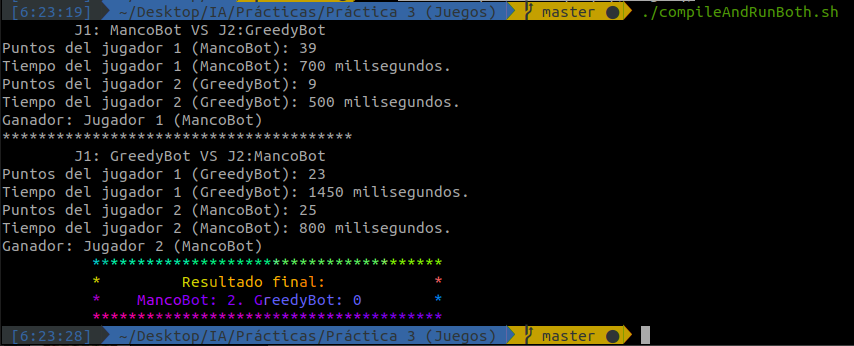
\includegraphics[scale=0.75]{mancovsgreedy.png}
\caption{Partidas contra \emph{GreedyBot}}
\end{figure}

\begin{figure}[H]
\centering
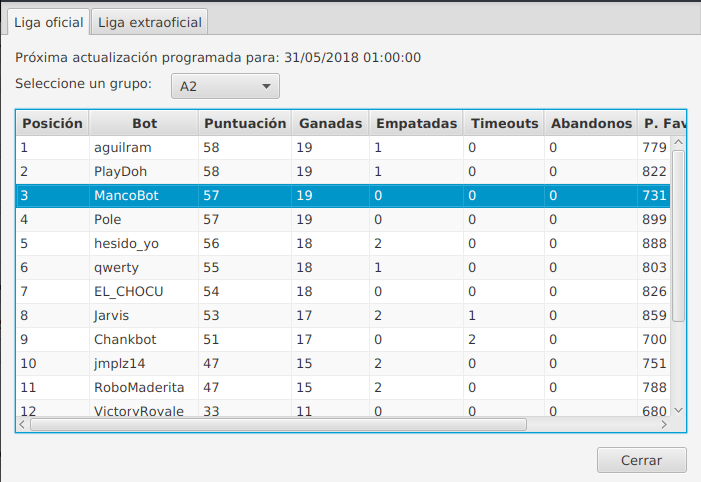
\includegraphics[scale=0.75]{liga.png}
\caption{Estado de la liga oficial (29/05/2018)}
\end{figure}

\newpage
\section{Anexo I. Código fuente}

\cppcode{../MancalaEngine/MancoBot.h}
\captionof{figure}{Fichero de cabecera.}

\cppcode{../MancalaEngine/MancoBot.cpp}
\captionof{figure}{Fichero de implementación.}

\newpage


\section{Anexo II. Scripts desarrollados}

\script{../compileAndRun.sh}
\captionof{figure}{Script que compila el bot y ejecuta la interfaz gráfica.}

\script{../compileAndRunNoGUIJ1.sh}
\captionof{figure}{Script que compila el bot y ejecuta la interfaz textual contra GreedyBot siendo J1.}

\script{../compileAndRunNoGUIJ2.sh}
\captionof{figure}{Script que compila el bot y ejecuta la interfaz textual contra GreedyBot siendo J1.}

\script{../compileAndRunBoth.sh}
\captionof{figure}{Script que compila el bot y ejecuta la interfaz textual contra GreedyBot en ambas posiciones. Muestra la salida como un marcador coloreado.}

\end{document}
